
\begin{frame}
\frametitle{2. ~ Circle packings}

A \emph{\bfseries circle packing} is a collection of circles that are either disjoint or tangent.


\begin{center}
 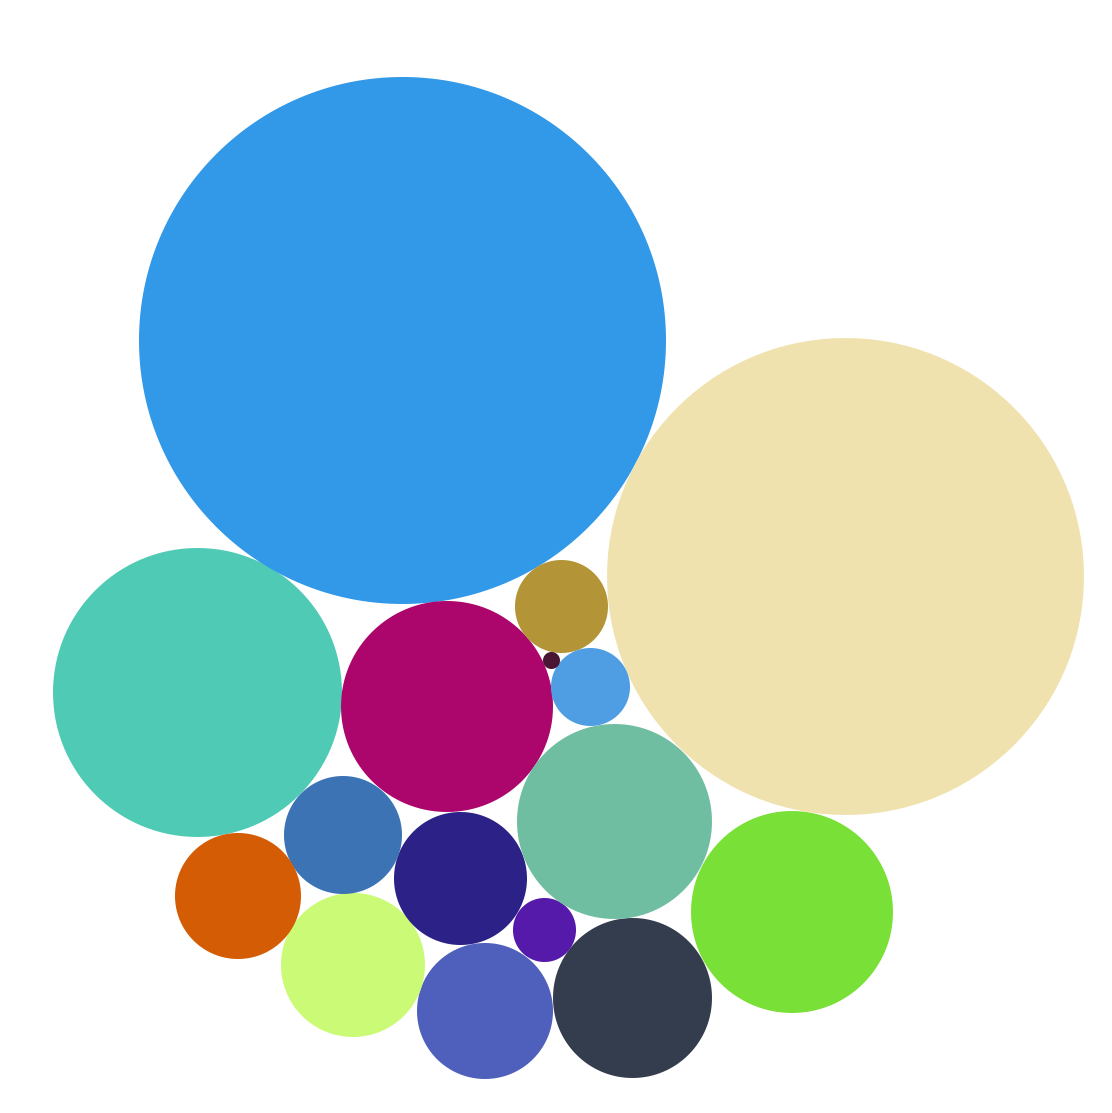
\includegraphics[width=180pt]{CP1.png}
\end{center}



\end{frame}




\begin{frame}
\frametitle{2. ~ Circle packings}


\begin{center}
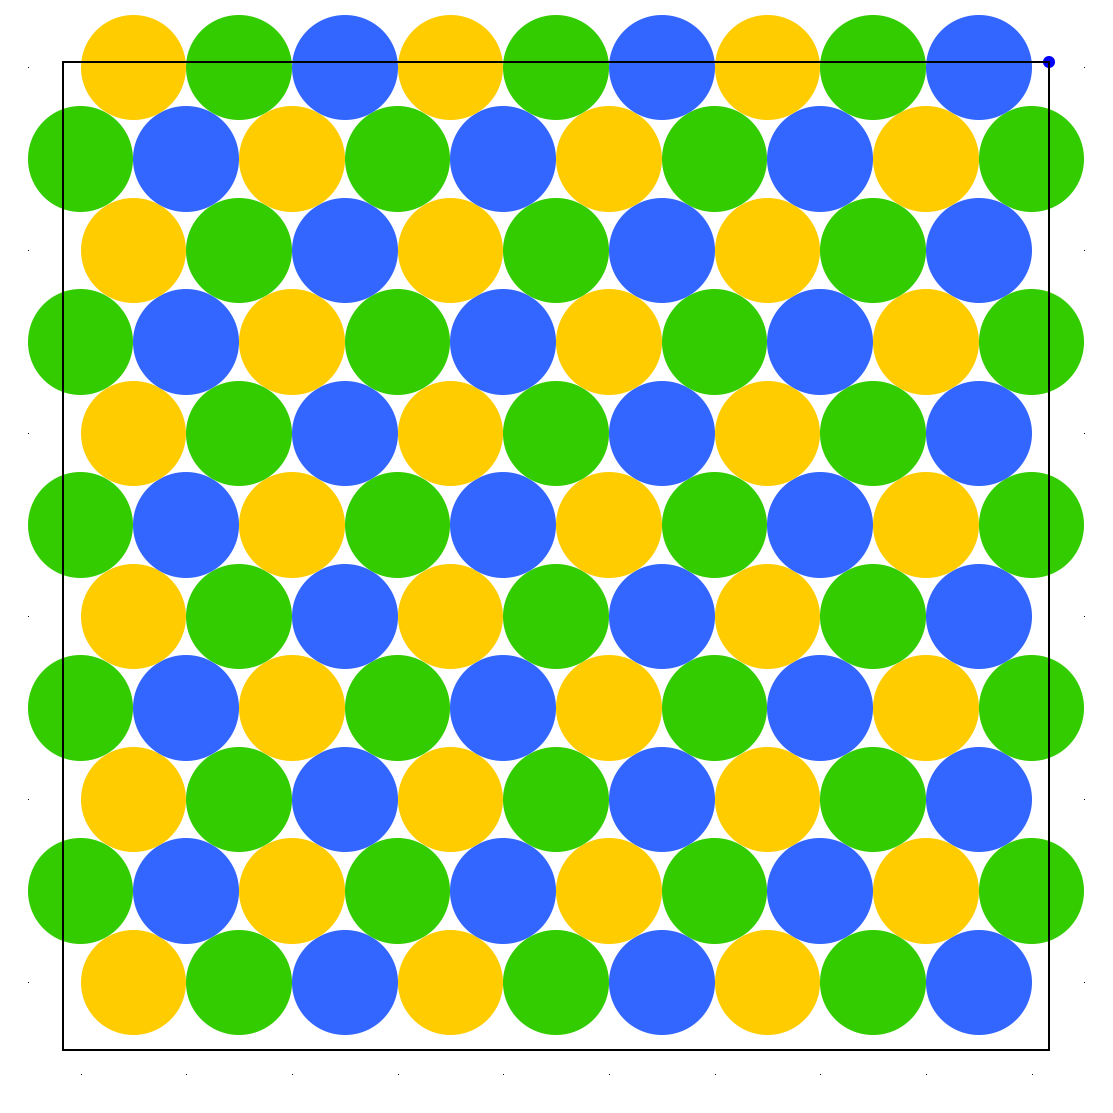
\includegraphics[width=130pt]{CP5.png} \hspace{30pt}
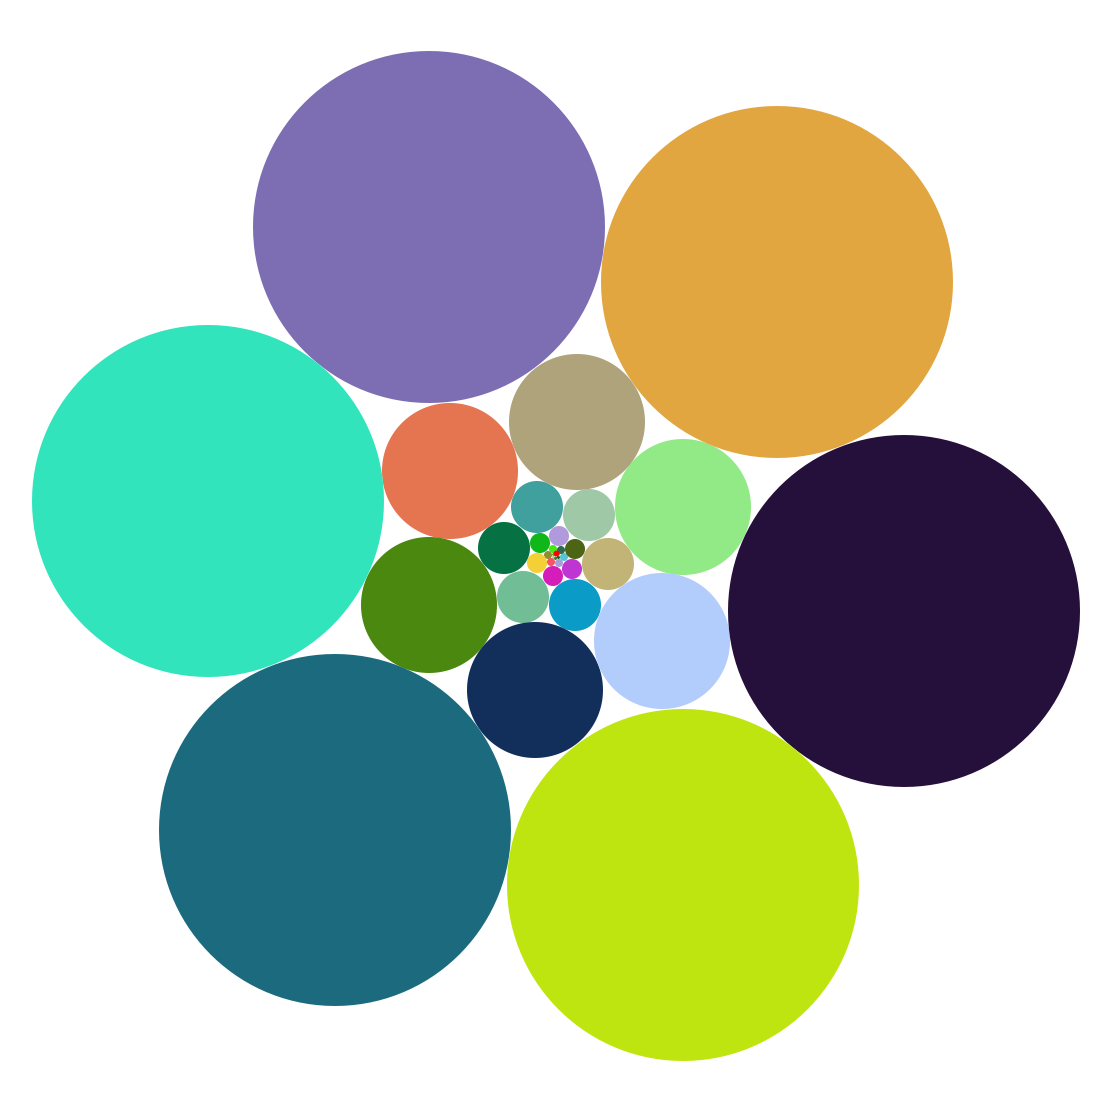
\includegraphics[width=130pt]{CP7.png}
\end{center}

\end{frame}






\begin{frame}
\frametitle{2. ~ Circle packings}



{\bfseries Appollonian gasket:}

\begin{center}
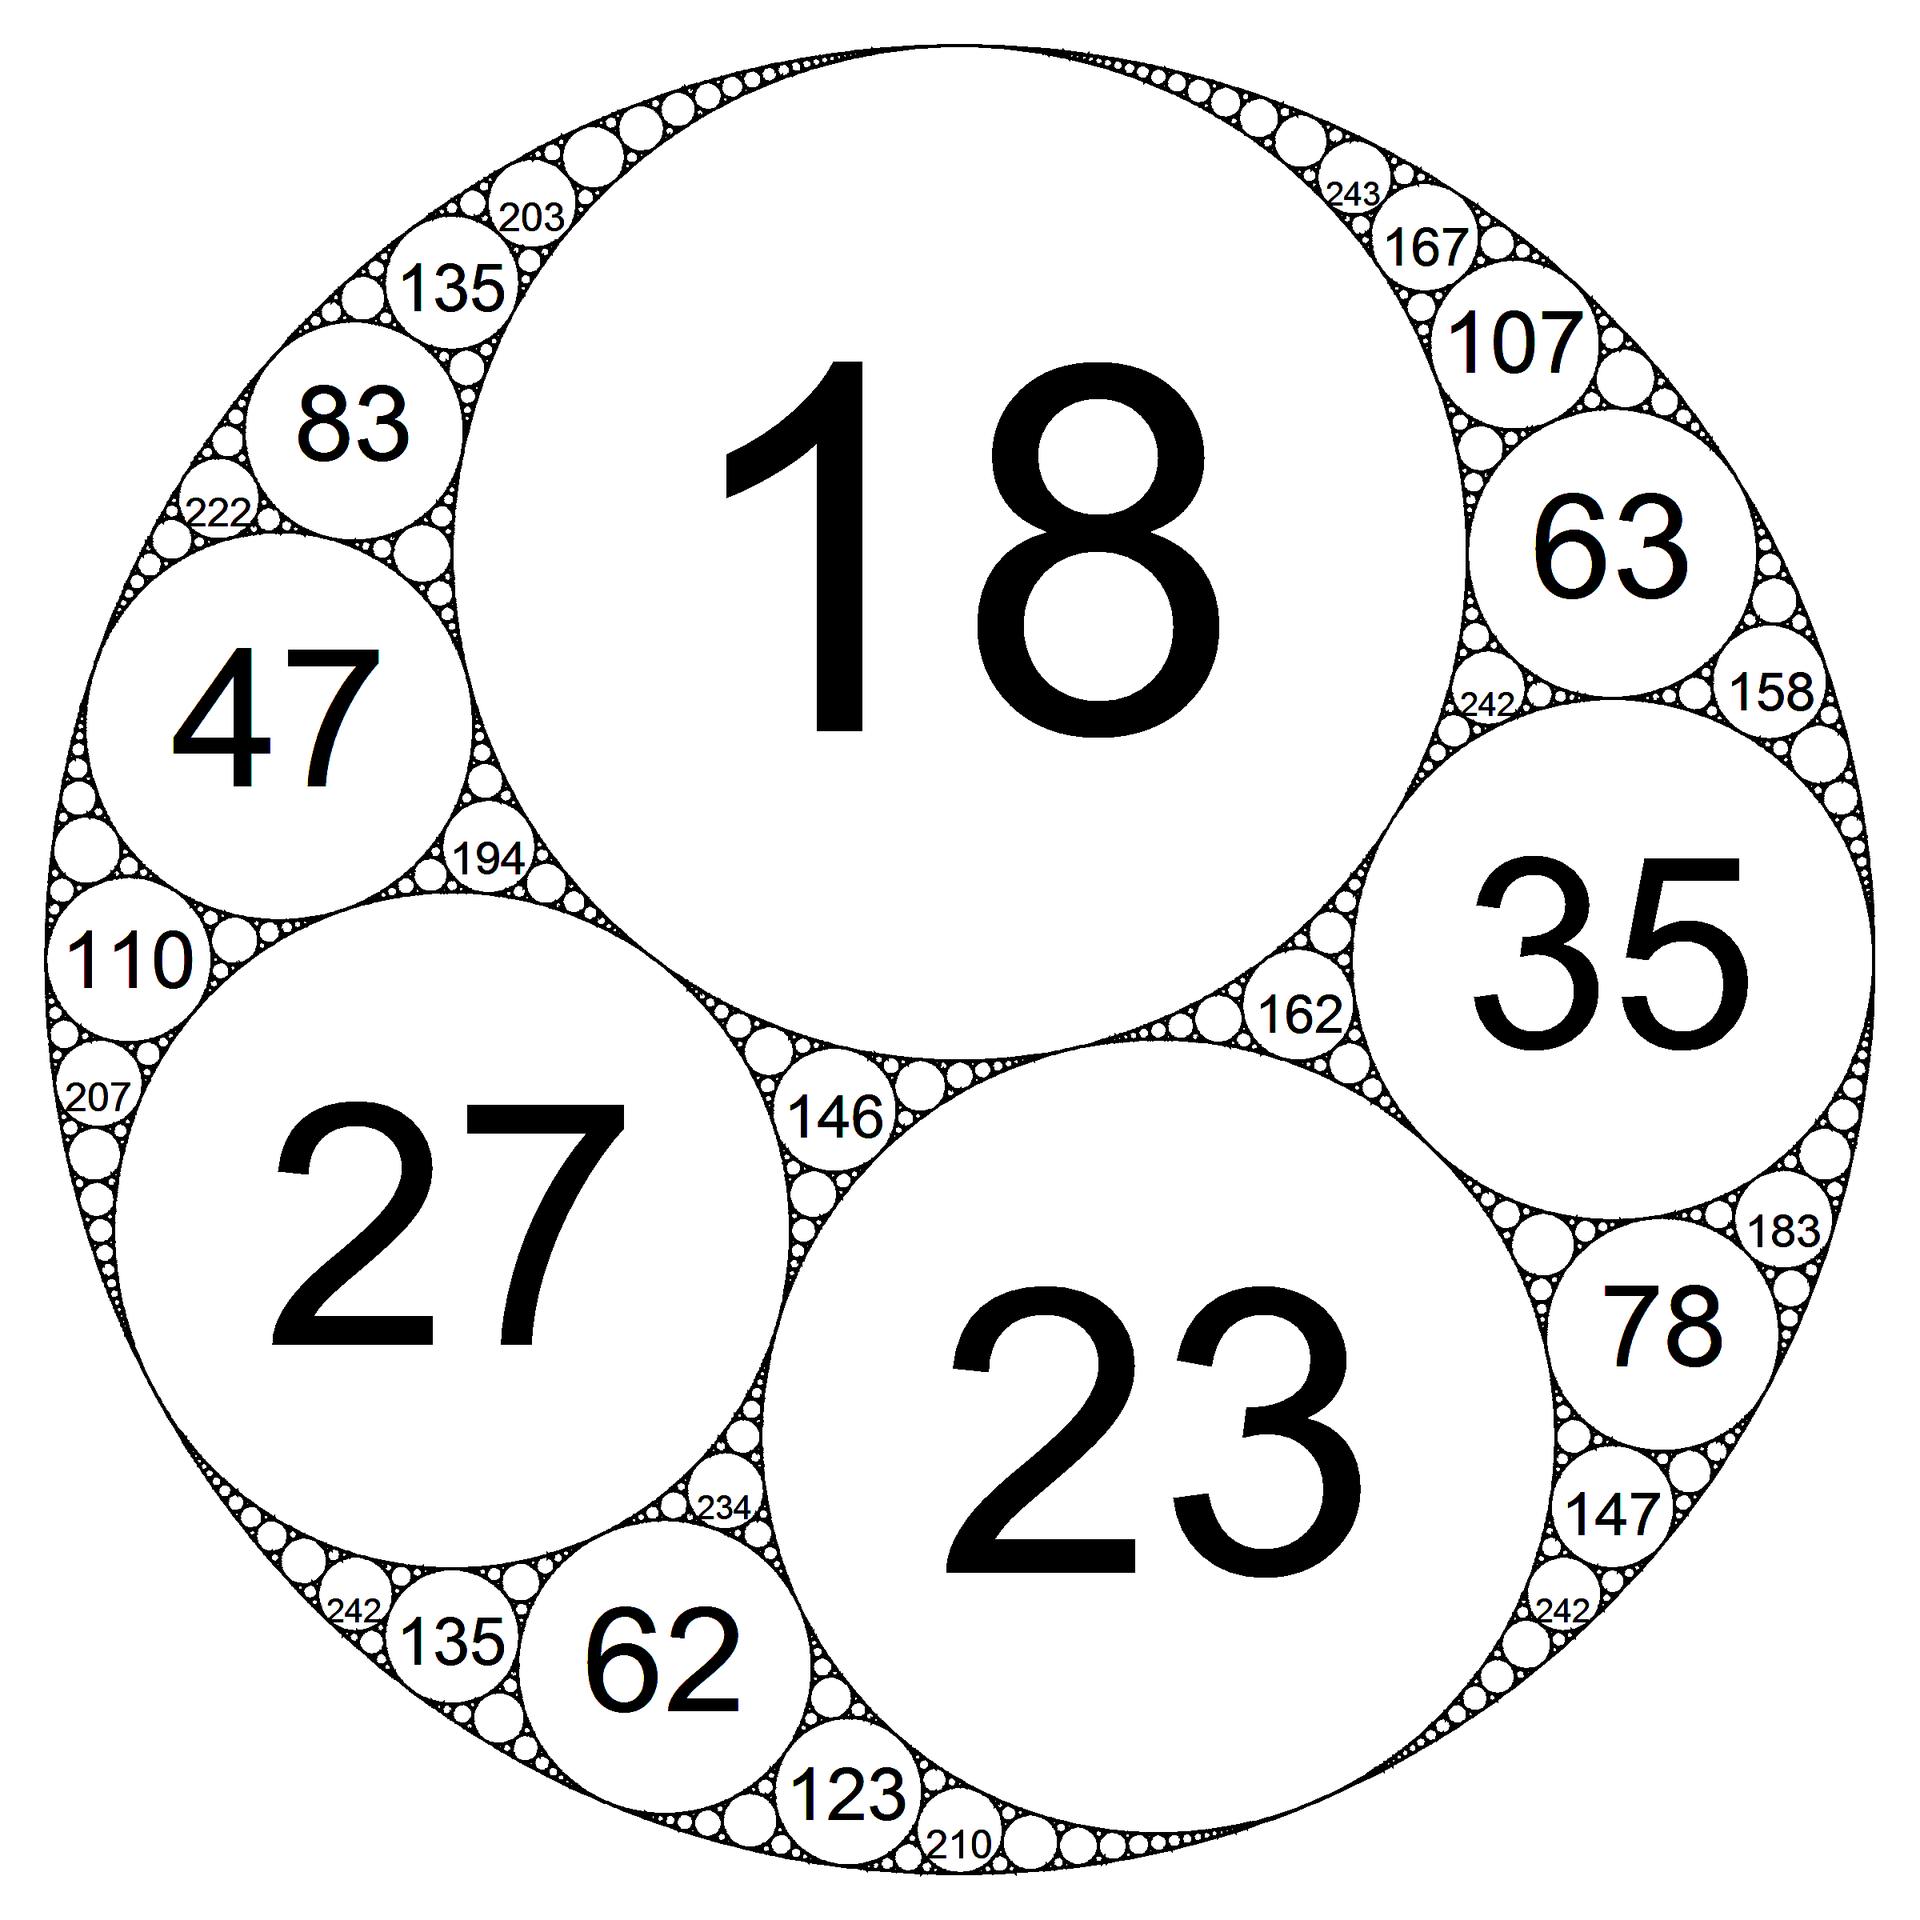
\includegraphics[width=170pt]{ApollonianGasket.png}
\end{center}

The curvatures (inverse radii) of four mutually tangent circles satisfy:
$(a + b + c + d)^2 = a^2 + b^2 + c^2 + d^2 $

\end{frame}
